\documentclass[tikz,border=2mm]{standalone}
\usepackage{tikz}
\usetikzlibrary{shapes.geometric, arrows, shapes.gates.logic.US, calc}

\tikzstyle{arrow} = [thick,->,>=stealth]

\begin{document}
    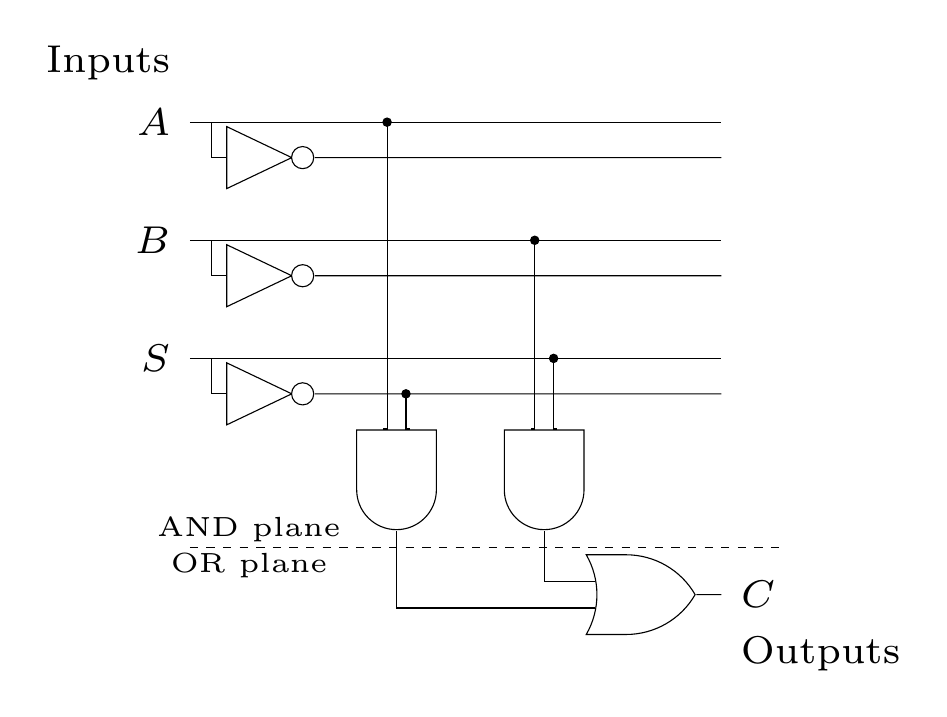
\begin{tikzpicture}[node distance=2cm, scale=1.5, every node/.style={scale=2}]

        % Inputs
        \node at (0,0.5) [left] (A) {\scriptsize Inputs};
        
        % A input with not gate
        \node at (0,0) [left] (A) {\scriptsize $A$};
        \draw (0, 0) -- (4.5,0);
        \node at (0.5,-0.3) [not gate US,draw](not) {};
        \draw (0.18, 0) |- (not.input);
        \draw (not.output) -- (4.5,-0.3);
        
        % B input with not gate
        \node at (0,-1) [left] (B) {\scriptsize $B$};
        \draw (0, -1) -- (4.5,-1);
        \node at (0.5,-1.3) [not gate US,draw](not) {};
        \draw (0.18, -1) |- (not.input);
        \draw (not.output) -- (4.5,-1.3);
        
        % S input with not gate
        \node at (0,-2) [left] (S) {\scriptsize $S$};
        \draw (0, -2) -- (4.5,-2);
        \node at (0.5,-2.3) [not gate US,draw](not) {};
        \draw (0.18, -2) |- (not.input);
        \draw (not.output) -- (4.5,-2.3);
        
        % AND plane
        \node at (0.5,-3.45) (S) {\tiny AND plane};
        \draw [dashed] (0, -3.6) -- (5, -3.6);
        
        % AND Gates
        \node at (1.75,-3) [and gate US, rotate=-90, logic gate inputs=nn,draw](and1) {};
        \node at (3,-3) [and gate US, rotate=-90, logic gate inputs=nn,draw](and2) {};
        
        % AND Connections
        % A NOT S
        \draw (1.67, 0) |- (and1.input 2);
        \filldraw[black] (1.67, 0) circle (1pt);
        \draw (1.83, -2.3) |- (and1.input 1);
        \filldraw[black] (1.83, -2.3) circle (1pt);
        
        % B S
        \draw (2.92, -1) |- (and2.input 2);
        \filldraw[black] (2.92, -1) circle (1pt);
        \draw (3.08, -2) |- (and2.input 1);
        \filldraw[black] (3.08, -2) circle (1pt);
        
        % OR plane
        \node at (0.5,-3.75) (S) {\tiny OR plane};
        
        % OR Gates
        \node at (3.75,-4) [or gate US, logic gate inputs=nn,draw](or1) {};
        
        % OR Connections
        \draw (and1.output) |- (or1.input 2);
        \draw (and2.output) |- (or1.input 1);
        
        % Output
        \node at (4.5,-4.5) [right] (A) {\scriptsize Outputs};
        \node at (4.5,-4) [right] (B) {\scriptsize $C$};
        \draw (or1.output) -- (4.5,-4);
            
        
    \end{tikzpicture}
\end{document}
